\section*{Paging: Two Advantages and Address Translation}
\begin{enumerate}
\item \textbf{flexibility}: support abstraction of address space: no need to assume direction of stack/heap growth and how they are used
\item \textbf{simplicity}: easy to manage free space: simply keep a list of free pages
\end{enumerate}
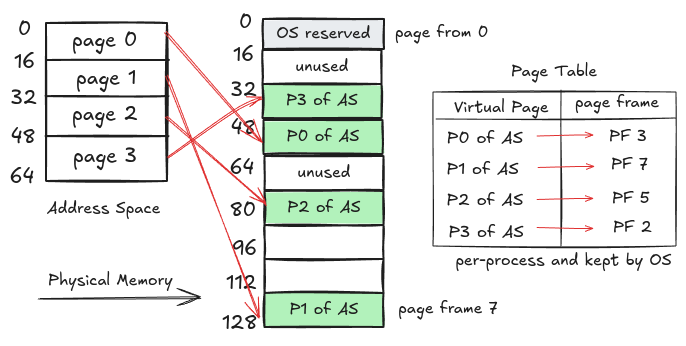
\includegraphics[width=\linewidth,height=4.5cm]{imgs/page_table}
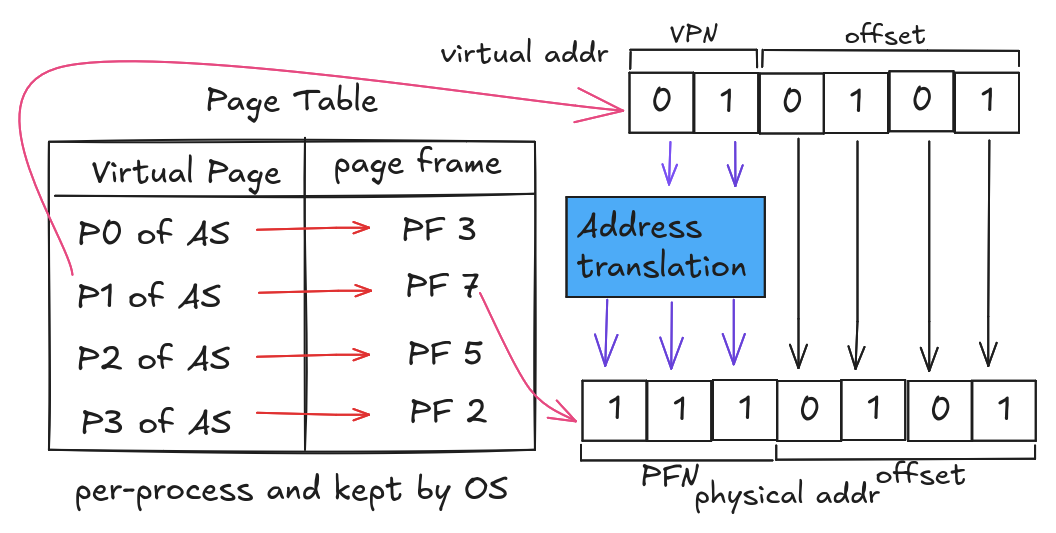
\includegraphics[width=\linewidth,height=4cm]{imgs/address_trans}
\section*{Page Table Issues: too big and too slow}
\begin{minipage}{0.5\linewidth}
  \flushleft
  \begin{itemize}
  \item 32-bit addr space, 4K pages: 20-bit VPN, 12-bit offset
  \item $2^{20} \approx 1$ million entries in page table for 1 process
  \item Assume each \textbf{PTE} needs 4B, 1 proc needs 4MB page table!
  \item Too big for MMU: physical memory or disk (by swapping page frams in/out of mem to disk)
  \end{itemize}
\end{minipage}
\begin{minipage}{0.5\linewidth}
  \begin{itemize}
  \item Extract VPN from virtual addr (VA) to find PFN
  \item Locate page table (e.g. in a page-table reg.)
  \item Compute addr of PTE for VPN
  \item Extract offset from VA and compute physical addr (PA)
  \item Fetch data from memory at PA
  \end{itemize}
\end{minipage}
\section*{Page Table Entry (PTE)}
Each PTE needs to store target PFN plus a few more information:
\begin{itemize}
\item valid bit: whether the VPN is mapped or not
\item protection bits: whether page is for read/write/code-execution
\item present bit: whether page is in memory or disk (swapped out)
\item dirty bit: page modified since it's brought to memory (swapping on)
\item reference bit: page has been accessed; for policies for page replacement
\end{itemize}
\section*{Accessing Memory With Paging}
\begin{lstlisting}[language=c]
VPN = (VirtualAddr & VPN_MASK) >> SHIFT    // get VPN from VA
PTEAddr = PTBR + (VPN * sizeof(PTE))        // compute PET addr
PTE = AccessMemory(PTEAddr)                 // fetch PTE
// Check if process can access the page
if (PTE.Valid == False)
  RaiseException(SEGMENTATION_FAULT)
else if (CanAccess(PTE.ProtectBits) == False)
  RaiseException(PROTECTION_FAULT)
else
  offset = VirtualAddress & OFFSET_MASK           // access ok
  PhysAddr = (PTE.PFN << PFN_SHIFT) | offset      // form physical addr
  Register = AccessMemory(PhysAddr)               // fetch it
\end{lstlisting}
